\chapter{Il ritorno di Ipparchia}

«Ippa! Ippa! Ipparchia!»\\
La sta chiamando forte, ma ancora non torna. Giovanni si siede sul muretto.

Dietro di lui, un edificio in rovina che non conosce perchè non ne ha ancora esplorato i dintorni. Giovanni ha tempo e lo usa come crede. Ora deve usarlo per attendere Ipparchia. Tiene il cartone sulle ginocchia.

Schopenhauer, ”L’arte di ottenere ragione”, stratagemma numero uno. Lo ripete tutto. Sa che sono passati circa trenta secondi. Se fosse stato un matematico, avrebbe contato, ma non era la matematica la sua passione.\\
Arriva allo stratagemma trentotto, è passato un’ora, e Ipparchia non è ancora tornata.

Dietro di lui, un luogo ignoto. Alla sua destra, la strada per il supermercato; a sinistra, la strada verso casa. Davanti, una via semi-inesplorata, ma la più probabile per ritrovare la cagnetta. Si incammina in quella direzione, continuando a chiamarla.

La strada diventa bianca: l’asfalto finisce, inizia la terra battuta. Da entrambi i lati, lo stesso fruscio tra gli alberi. Ogni quindici metri, un tronco più grande degli altri.

Quando Ipparchia lo ha lasciato erano circa le otto di sera, quindi ora è quasi buio. Per lui non cambia molto, ma i cani usano anche la vista.\\
Arriva a un incrocio: la strada bianca curva a destra, mentre dritto torna asfaltata.\\
«Ippa! Dove sei andata?»

Giovanni tiene la destra e si addentra in campagna. Gli alberi continuano a costeggiare la strada, ne conta nove, poi all’improvviso l’asfalto ritorna.

\par\medskip
\begin{center}
  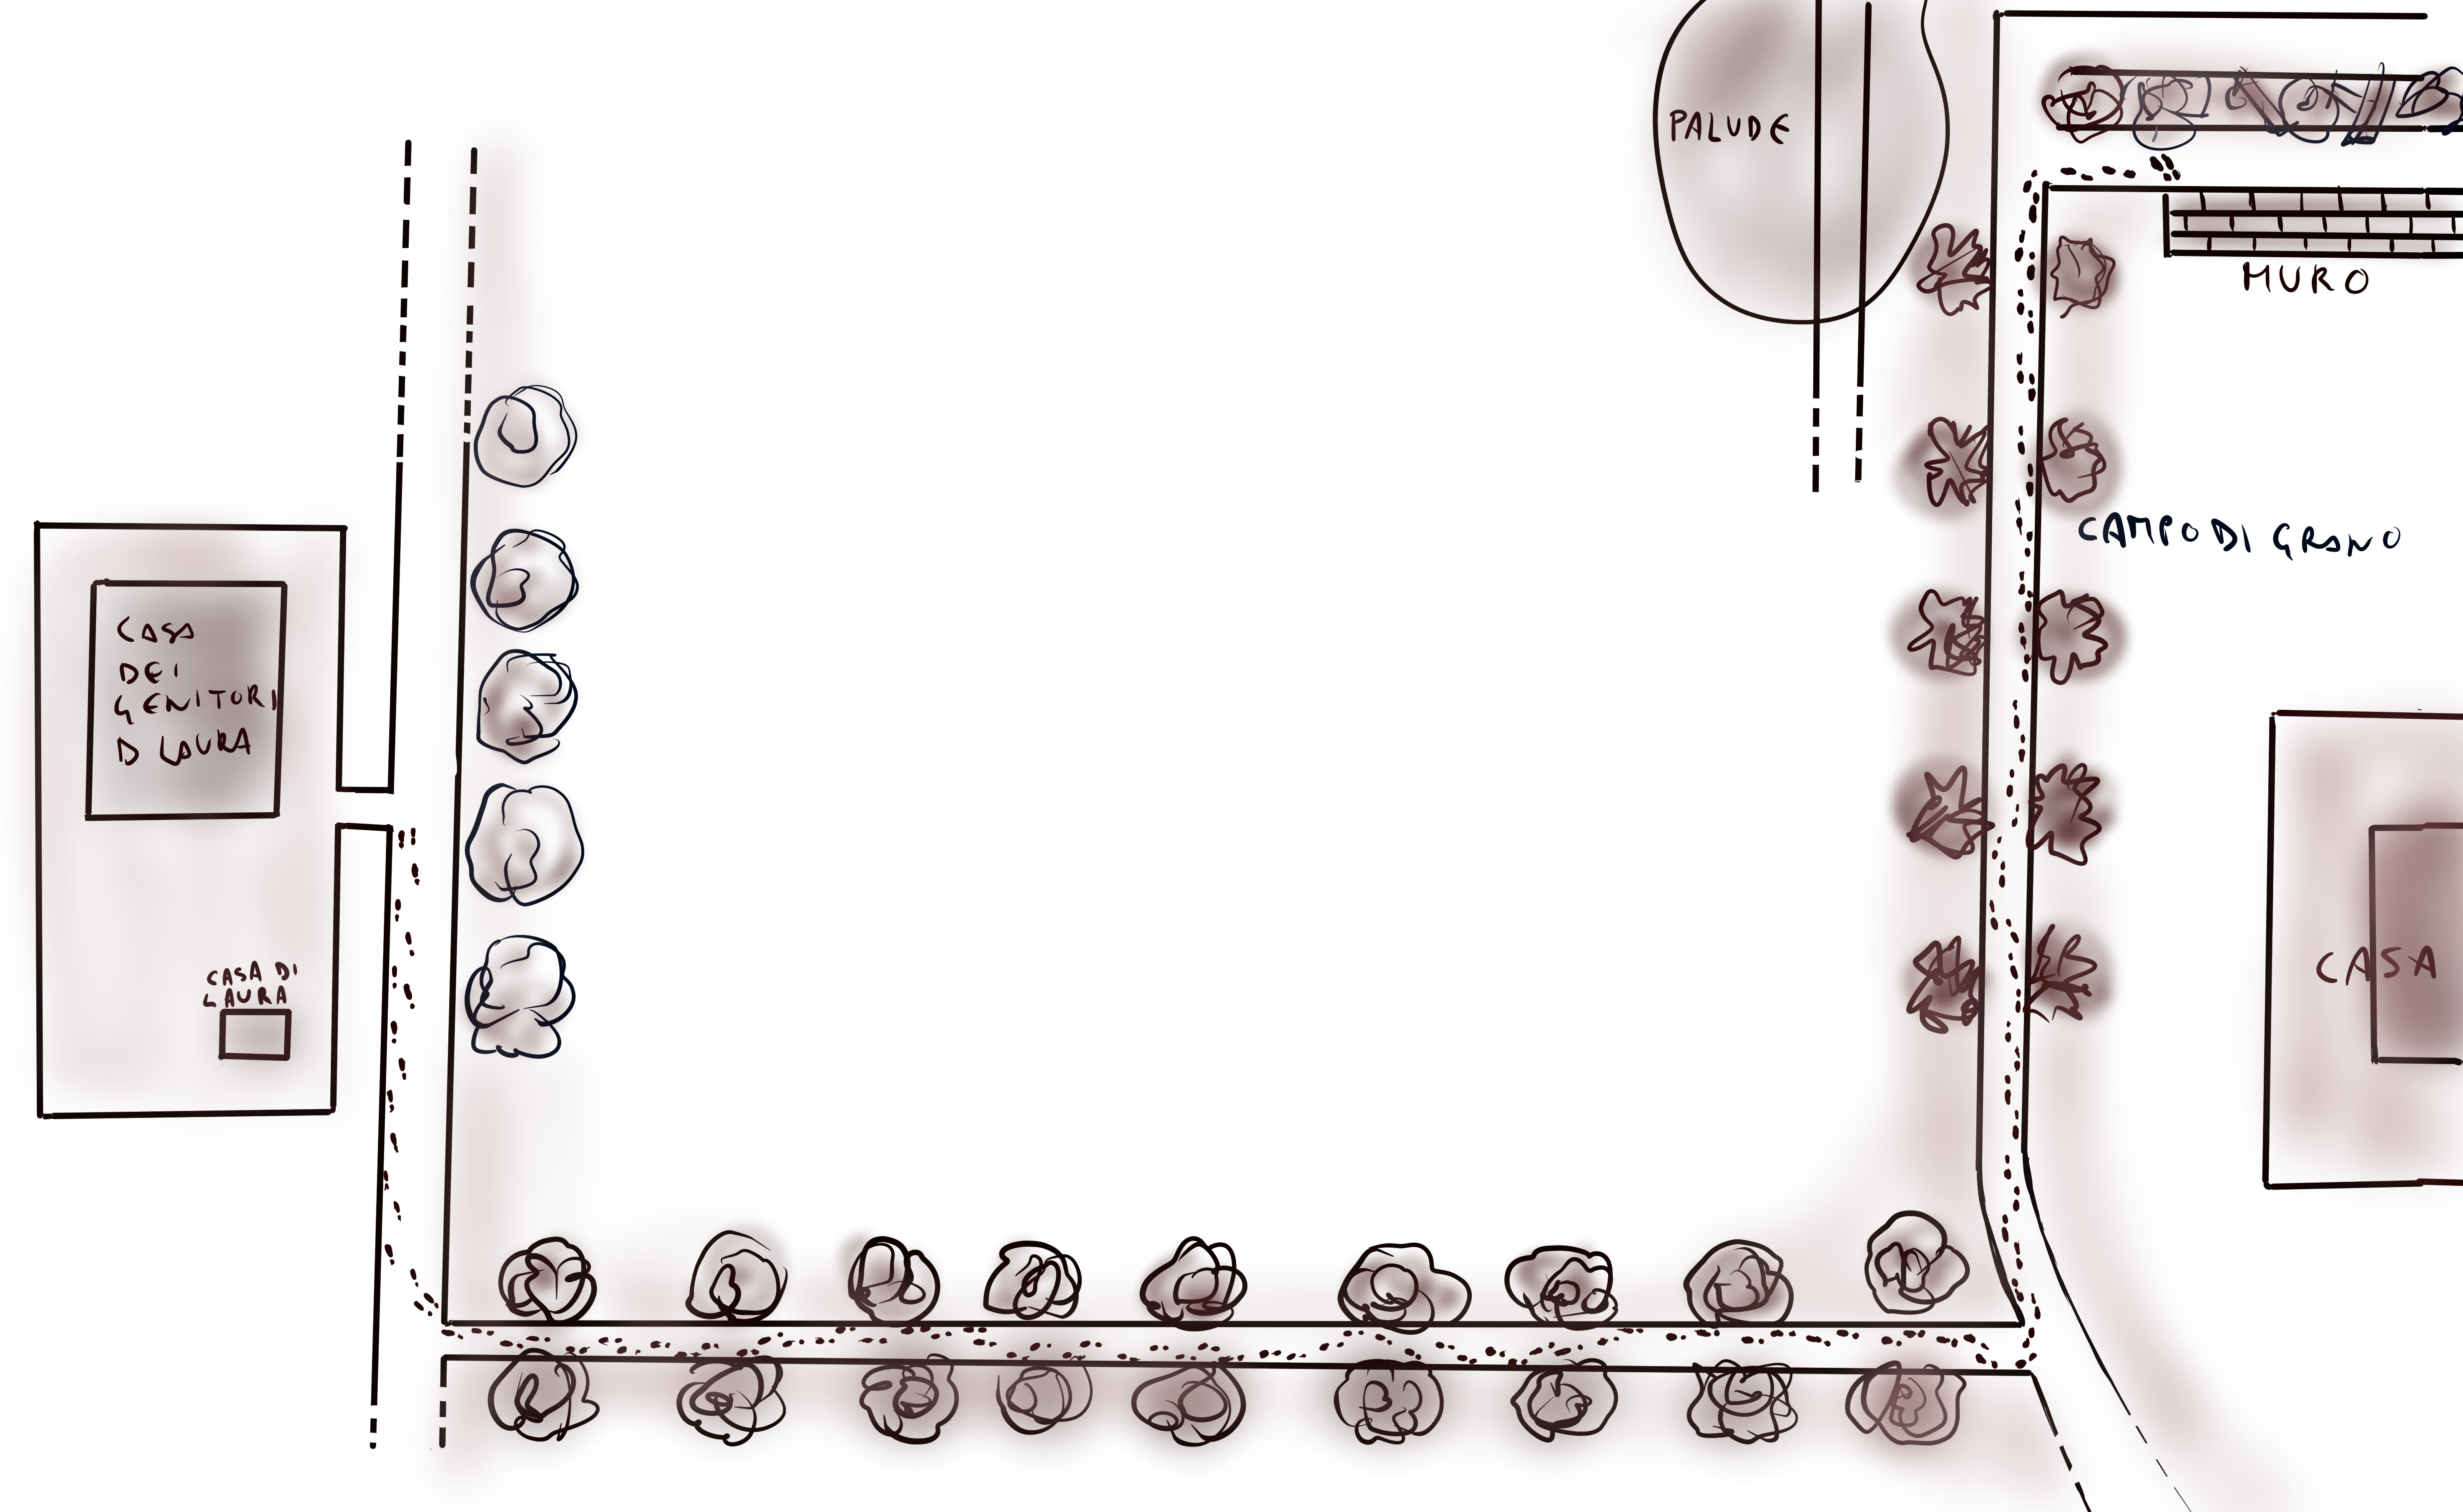
\includegraphics[width=0.9\linewidth]{mappa con casa laura.png}
\end{center}

Attende qualche minuto. Sente passare un veicolo. La strada che ha incontrato taglia quella bianca: deve essere una vecchia via di comunicazione.

Sta per tornare indietro, quando dall’altra parte della strada una voce familiare lo fa voltare:\\
«Ippa!»\\
Attraversa senza esitazione.\\
«Ippa!» Le va incontro, lei rimane ferma, la raggiunge e capisce cosa è successo: il guinzaglio di corda è rimasto incastrato in qualche anfratto, ma Giovanni la libera facilmente.

Ipparchia lo lecca, ma… sono due le lingue. Un altro cane è accanto a lei.\\
«C’è un altro cane qui...» chiama più volte: «C’è un cane qui! E’ di qualcuno questo cane?»\\
Nessuna risposta.

«Andiamo, Ippa.»\\
Ripartono e sul tratto asfaltato il rumore è quello di otto zampe.\\
Raggiungono di nuovo la strada bianca. Giovanni si inginocchia e accarezza il nuovo arrivato.\\
«E tu? Ci segui?» Si gratta la testa. «In ogni caso, non saprei come altro aiutarti per ora. Va bene, andiamo a casa, poi vedremo.»

Ripercorre la strada dell’andata, passo dopo passo, rumore dopo rumore, odore dopo odore.\\
«Coraggio, è tardi, ma si va a cena.»

Giovanni regge il pacco per le ultime decine di metri che lo separano dal rifugio.\\
L’odore delle rose dell’ultima abitazione si mescola alla lavanda spontanea che cresce nel parco abbandonato dell’ex convitto.\\
Avanza tra spine di more e ciuffi di rosmarino, che pungono le gambe e coprono l’odore di Ippa e dell’altro cane. Un dedalo verde che è la sua protezione segreta.

Le braccia gli pesano, ma ormai ce l’ha fatta.\\
Un ramo si spezza a pochi metri:\\
«Ehi, c’è qualcuno?»\\
Silenzio. Nulla di strano, forse solo un ramo secco.

Manca solo da salire la scala antincendio quando, alle sue spalle, una voce lo ferma:\\
«…Appoggia il pacco, amico.»

Giovanni resta immobile.\\
«Mi hai trovato.» Lo dice lentamente, a sentirlo sembrerebbe il copione di un film, tipo Sergio Leone.\\
Lentamente, posa il pacco sul primo pianerottolo e impercettibilmente lascia scorrere la mano verso il fianco.\\
«Io non lo farei…» la voce è leggermente coperta da Ipparchia e il nuovo compagno che ringhiano sommessamente, il pelo irto, lo sguardo fisso verso il buio alle sue spalle.\\
«Tu non sei me, perchè tu sei…»

Un passo nel buio. Qualcosa striscia tra le foglie secche, appena oltre il cerchio di luce.

Giovanni stringe le mascelle.

Ipparchia e l’altro cane ringhiano più forte, le zampe piantate a terra.

Poi la voce, ferma e bassa:

«… un uomo morto.»

Un colpo secco, come di legno che batte sul metallo, rompe il silenzio.
